\documentclass[letterpaper,12pt]{article}
\usepackage{tabularx} % extra features for tabular environment
\usepackage{amsmath}  % improve math presentation
\usepackage{graphicx} % takes care of graphic including machinery
\usepackage[margin=1in,letterpaper]{geometry} % decreases margins
\usepackage{cite} % takes care of citations
\usepackage{longtable}
\usepackage{booktabs}
\usepackage[final]{hyperref} % adds hyper links inside the generated pdf file
\hypersetup{
	colorlinks=true,       % false: boxed links; true: colored links
	linkcolor=blue,        % color of internal links
	citecolor=blue,        % color of links to bibliography
	filecolor=magenta,     % color of file links
	urlcolor=blue         
}
\usepackage{gensymb}
\usepackage{blindtext}
%++++++++++++++++++++++++++++++++++++++++


\begin{document}

\title{Robotics and Deep Learning}
\author{Michele Antonazzi}
\date{\today}
\maketitle

\begin{abstract}
This work is an overview concerning robotics and the machine learning applications can have on it, with a particular focus on deep learning.  
\end{abstract}

\section{Introduction}\label{header-n3}

In the last few years, advances in technologies and research have had a
great impact on the development of robotics. The robots are employed
every day in a large variety of contexts. They substitute humans in
those activities that can be performed more quickly and precisely. An
example is manufacturing when the production process is automatized
using artificial agents to improve productivity and reduce costs. In
this case, the robots are fixed manipulators with a limited range of
motions, that depends on where it is bolted down. This characteristic
strongly limits the agent's possibilities. Generally, a fixed robot is
programmed to perform a single precise task and it operates in a
controlled environment. This means that the algorithm foresees every
possible situation and often it is coded as a state machine. In
contrast, mobile robots would be able to travel within the environment
in which they operate, applying their talents wherever it is most
effective. Thank mobility, the robotics applications become almost
limitless. Some of them are healthcare, entertainment, and rescue.
Mobile robots are also employed in those tasks that are impossible or
too dangerous for humans, as the exploration of hostile environments: a
building on fire, the seabeds, or the surface of another planet. These
robots can be controlled by humans or can be autonomous. The firsts are
controlled through remote controls while the seconds perceive the
environment and move autonomously according to their task, without human
intervention. The main problem that a mobile robot has to solve is how
to move inside the environment. The first aspect is the \emph{motion
	control}. Each robot has a different locomotion system, specific for the
characteristics of the environment in which it moves. Given its
low-level complexity, the motion actions are performed by a specific
software component. To perform the motion control task is necessary to
use the kinematics: the study of how the robot's mechanical systems
behave. To define the kinematics of a robot, it is necessary to define a
geometrical model (specific for the mechanical characteristics of the
locomotion system) that allows expression of robot motion in a global
reference frame and in the robot's local reference frame. Using this
notation, it is possible to define the robot's kinematics model that
describes the movements and their constraints as a function. Through
kinematics, it is resolved the significant challenge of \emph{position
	estimation}. The next step is the \emph{perception}. An autonomous
system has to acquire knowledge about the environment. This is done by
taking measurements using various sensors and then extracting
information from those measurements. With this information, a mobile
robot can determine its position in the environment. This activity is
called \emph{localization}. The last step for an autonomous mobile agent
is \emph{navigation}. Given partial knowledge about its environment and
a goal position or a series of positions, navigation is the ability of
the robot to act based on its knowledge and sensor values to reach its
goal positions as efficiently and as reliably as possible. There are two
main sub-task of navigation: \emph{path planning} and \emph{obstacle
	avoidance}. The first involves identifying a trajectory that will cause
the robot to reach the goal location when executed. The second consists
of modulating the trajectory of the robot in order to avoid collisions.
Using the techniques explained before, an autonomous mobile robot is
able to robustly navigate inside an environment to perform its tasks.
However, a mobile robot operates in a highly non-deterministic context
and the conventional algorithms often are not suitable or not robust
enough. In the real world, in fact, there are a lot of different tasks
that are too complicated to be modeled by a conventional algorithm. Some
problems indeed may have a wide amount of data difficult to analyze. In
this case, build a specific algorithm means to understand the complex
patterns and the hidden correlations between the data. Instead, other
tasks may be influenced by a lot of external factors that generate a
large quantity of similar but different data. These factors are not easy
to model, especially considered all together, and often they are not a
priori known. This means that an algorithm performs well only in a
controlled environment, that respects specific preconditions. On the
other hand, if it is applied in the real world, the algorithm may
encounter data that it cannot correctly analyze. A particular field of
Computer Science is particularly suitable to solve these situations:
\emph{machine learning} (ML). It represents a family of algorithms that
learn automatically through experience. These algorithms are not
designed for a specific task but they are general purposes so they can
be used to solve each type of task. The principle behind machine
learning is the following: each real phenomenon can be modeled as an
unknown mathematical function which can be approximate by a machine
learning algorithm. In this work, the focus is posed on \emph{deep
	learning} and its application to robotics. Deep learning is based on
artificial neural networks, inspired by the biological neural network
that composed the animal brains. In the following sections are resumed
some papers that apply deep learning to robotics. Each of them specifies
the article title, the name of the journal where it has been published,
and the publication year. For each article is summarized the approach
proposed, the innovation with respect to the literature and the
achievements.
\newpage

\section{The limits and potentials of deep learning for
robotics}\label{header-n5}

\emph{THE INTERNATIONAL JOURNAL OF ROBOTICS RESEARCH 2018, Vol. 37(4--5)
405--420} {[}1{]}

\subsection{Introduction}\label{header-n7}

A robot is an inherently active agent that interacts with the real world
and often operates in uncontrolled or detrimental conditions. Mistakes
can lead to potentially catastrophic results, like put human lives at
risk, e.g. if the robot is a driverless car. The application of deep
learning in robotics, therefore, motivates research questions that
differ from those typically addressed in other domains. How much trust
can we put in the predictions of a deep learning system when
misclassifications can have catastrophic consequences? How can we
estimate the uncertainty in a deep network's predictions and how can we
fuse these predictions with prior knowledge and other sensors in a
probabilistic framework? How can we generate enough high-quality
training data? We can obtain these data in real-world scenarios or we
can obtain them using data augmentation through simulation? Is there a
fundamental difference between model-driven and data-driven
problem-solving? This paper explores some of the challenges, limits, and
potentials for deep learning in robotics.

\subsection{Challenges for deep learning in robotic
vision}\label{header-n9}

\begin{figure}[h!]
	\centering
	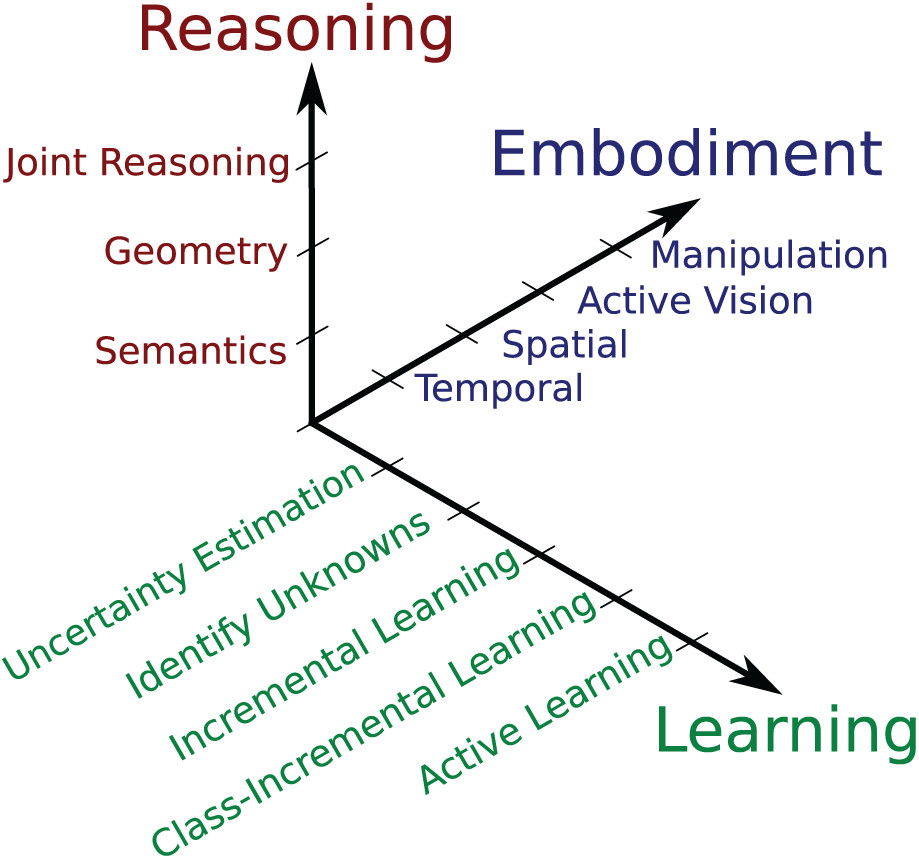
\includegraphics[width=0.5\linewidth]{images/roboticvision.jpeg}
	\caption{Current challenges for deep learning in robotic vision}
\end{figure}

\emph{Robotic vision} differs from \emph{computer vision} in several
aspects. In particular, the latter is a part of the first. A robot is an
active agent that perceives the world with its different sensors, builds
a coherent model of the world, and updates this model over time, but
ultimately a robot has to make decisions, plan actions, and execute
these actions to fulfill a useful task. In fact, for robotic vision,
perception is only one part of a more complex system. In a simplified
view, whereas computer vision takes images and translates them into
information, robotic vision translates images into actions. This
fundamental difference between robotic vision and computer vision
motivates a number of research challenges along three conceptually
orthogonal axes: \emph{learning}, \emph{embodiment}, and
\emph{reasoning}. We position individual challenges along these axes
according to their increasing complexity, and their dependencies.



\subsubsection{Learning challenges}\label{header-n12}

Along this axis, we position challenges that are specific for (deep)
machine learning in a robotic vision context.

\paragraph{Uncertainty estimation}
It is important that deep learning systems can reliably estimate the
uncertainty in their predictions. The robot has to treat a neural
network in the same way as other sensors, also using Bayesian techniques
to fuse the network's predictions with prior knowledge to accumulate
information over time. Typically a deep learning model returns scores
that are not calibrated probabilities so not useable in a Bayesian
sensor fusion framework. 
\paragraph{Identify unknowns}

A common assumption in deep learning is that trained models will be
deployed under \emph{closed-set} conditions. However, robots often have
to operate in ever-changing, uncontrolled real-world environments, and
they will inevitably encounter data not covered by the training data. In
these \emph{open-set} conditions, it is crucial to identify unknowns
with high confidence.
\paragraph{Incremental learning}

A robotic vision system should be able to learn from new training
samples of known classes during deployment, upgrading its internal
representations accordingly.

\paragraph{Class-incremental learning}

A robot, therefore, needs the capability to extend its knowledge and
efficiently learn new classes of interest without forgetting the
previously learned ones. Current techniques for class-incremental
learning still rely on supervision in the sense that the user has to
specifically tell the system which samples are new data.

\paragraph{Active learning}

A robot should be able to select the most informative samples for
incremental learning techniques on its own. In order to minimize the
interaction with the humans, the robotic system can also comprise
retrieving annotations from other sources such as the web.

\newpage
\subsubsection{Embodiment challenges}\label{header-n24}

\paragraph{Temporal embodiment}

A robotic vision system perceives a stream of consecutive and therefore
strongly correlated images. The potential of temporal embodiment to
improve the quality of the perception process for object detection or
semantic segmentation is currently rarely utilized. A robotic vision
system that uses its temporal embodiment can, for example, accumulate
evidence over time or exploit small viewpoint variation. A challenging
aspect of the temporal embodiment is that the appearance of scenes
changes over time. An environment can comprise dynamic objects which
move inside it. Besides, an environment can also change its appearance
according to different lighting conditions (day/night), structural
changes in objects (summer/winter).

\paragraph{Spatial embodiment}

The camera of a robotic system is spatially embodied and it will observe
the scene according to the robot's movements. This fact poses both
challenges and opportunities to a robotic vision system: it can help to
disambiguate its semantic properties, improve depth perception, or
segregate an object from other objects or the background in cluttered
scenes. On the other hand, occlusions can alter or changes the visual
perception.

\paragraph{Active vision}

One of the biggest advantages of a robot is the potential to control the
camera, move it, and change its viewpoint independently from the robot's
movements. In this way, a dynamic robotic vision system can improve its
perception confidence, resolve ambiguities, and mitigate the effect of
occlusions or reflections.

\paragraph{Manipulation for perception}

As an extension of active vision, a robotic system could manipulate the
scene to improve its perception. For example, a robot could move
occluding objects or move an object to see its occluded faces.

\subsubsection{Reasoning challenges}\label{header-n33}

Von Helmholtz (1867) formulated the idea that humans use unconscious
reasoning when processing visual information, in order to inference
concepts or make conclusions. The following searches investigate these
unconscious mechanisms and reformulated them in a Bayesian inference
framework.

\paragraph{Reasoning about object and scene semantics}

The world around us contains many semantic regularities that humans use
to aid their perception: objects tend to appear more often in a certain
context, some objects tend to appear in groups, some objects rarely
appear together in a scene, and so on. If these semantic regularities
can be used by a vision system as prior knowledge, we can expect an
improved and more robust vision framework.

\paragraph{Reasoning about object and scene geometry}

Many applications in robotics require knowledge about the geometry of
individual objects, or the scene as a whole. Estimating the 3D structure
of scenes or objects from multiple views without having depth
information is a widely researched topic. A robot, differently from a
classical approach, has to perform this task in cluttered scenes, where
the objects are not clearly separated. A robot needs the ability to
express uncertainty in the inferred object shape and it should be able
to exploits its embodiment to move the camera to collect new and more
useful information. Inference over the geometry of the whole scene is
related also to object-based simultaneous localization and mapping
(SLAM).

\paragraph{Joint reasoning about semantics and geometry}

The final reasoning challenge for a robotic vision system, therefore, is
the ability to reason jointly about the semantics and the geometry of a
scene. Semantics and geometry can help each other: a tightly coupled
inference approach can be advantageous compared to two systems that work
separately.

\subsection{The evaluation method for deep learning models applied to
robotics}\label{header-n41}

Normally the good deep learning performance is not reached when the
models are used in real environments. The evaluation method used in
computer vision fails when applied in robotics: a robot has to interact
with a dynamic environment and not with a simple set of images
downloaded from the Internet. When a statistic report indicates that a
dataset has been solved, it does not necessarily mean that the problem
itself has been solved. The available datasets often are not able to
able to correctly evaluate the performance of a robotic deep learning
model. One of the reasons is the datasets' inability to give to the
model information about the unknowns aspect of real environments. In
particular, \emph{Open set recognition} refers to scenarios where
incomplete knowledge of the world is present at training time. This
implies that unknown classes can be submitted to the model during its
operation. What is needed is a new class of machine learning algorithms
that minimize the risk of the unknown. To do this, updated evaluation
protocols are also needed. These protocols have to incorporate data that
is both know and unknown to a model. Another important aspect is the
systematic study of the performance of a recognition model across an
exhaustive range of object appearances. To better understand this
mechanisms, inner in the humans' visual system, psychophysics discipline
can be used. Psychophysics investigates the relationship between
physical stimuli and the sensations and perceptions they produce. This
concept can be translated into the field of deep learning: we would like
to know under what conditions a machine learning model is able to
operate successfully, as well as where it begins to fail. But how
exactly can Psychophysics be applied to deep models? One possibility is
through a computational pipeline that is able to perturb the data at a
massive scale (e.g. millions of images per image transformation being
studied) and submit them to a model, studying its performance through
the item--response curve. The key to interpreting the results is the
ability to identify the model's preferred view. The preferred view
concept derives from vision science, which has established that humans
possess an internalized canonical view (the visual appearance that is
easiest to recognize) for individual object classes. Similarly,
recognition models have one or more preferred views of an object class,
each of which leads to a maximum (or minimum) score output. The
psychophysics progresses support a growing trend in robotics and
computer vision: simulation using rendered graphics. The models'
performance can be assessed by comparing the respective item--response
curves. Importantly, this technique can find potential gaps not only
between different models but also between human and model behavior.
Human performance vastly exceeds model performance even in cases where a
problem has been assumed to be solved, especially comparing the
item-response curves.

\subsection{The role of simulation for pixel-to-action
robotics}\label{header-n43}

\emph{Deep reinforcement learning} is a new learning paradigm that is
capable of learning end-to-end robotic control tasks, but its results
have been demonstrated primarily in simulation, rather than on real
robot platforms. Demonstrating learning capabilities on real robots
remains a significant challenge: the long, data-hungry training paradigm
of pixel-based deep robotic learning methods are too computationally
hard to be executed by a robotic platform. On the other hand, in
simulation, the training time can be greatly reduced by using dedicated
hardware and parallelism paradigms. Another important difference that
often separates a simulated task and its real-world analog concerns raw
pixel inputs. One solution is to use transfer learning methods, but
there exist fewer approaches for transfer from simulation to reality for
robot domains. Another one consists of augmenting the target
domain data with data from the source domain. Another approach is to use
a ``confusion" loss that forces the model to ignore data variations that
separate the two domains. A more recent simulation-to-real solution
relies on the \emph{progressive network} architecture, which enables
transfer learning through lateral connections that connect each layer of
previously learned deep networks to new networks to model the gap
between the two domains. 
\begin{figure}[h!]
	\centering
	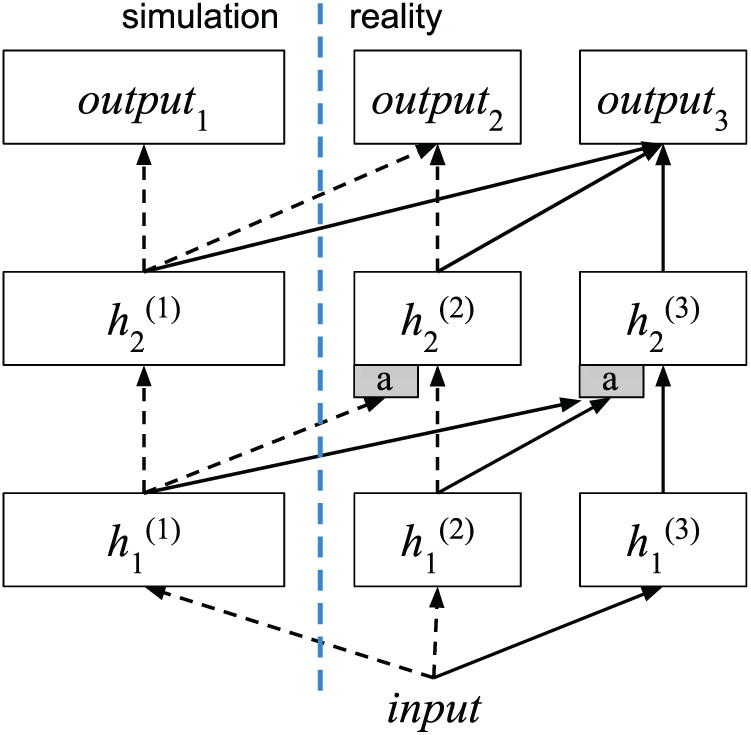
\includegraphics[width=0.5\linewidth]{images/progressivenets.jpeg}
	\caption{Detailed schematic of progressive recurrent network architecture}
\end{figure}

The progressive networks advantages for
simulation-to-real transfer are the following:

\begin{itemize}
\item
  the features learned for one task may be transferred to many new
  tasks;
\item
  the columns may be heterogeneous, which may be important for solving
  different tasks, including different input modalities, or simply to
  improve learning speed when transferring to the real robot;
\item
  progressive nets add new capacity, including new input connections,
  when transferring to new tasks. This is advantageous for bridging the
  reality gap, to accommodate dissimilar inputs between simulation and
  real sensors.
\end{itemize}



\subsection{Deep learning and physics-based models}\label{header-n53}

The predominant approach to perception, planning, and control in
robotics is to use approximate models of the physics underlying a robot,
its sensors, and its interactions with the environment. These models
require that their parameters are known with sufficient accuracy and can
be tracked over time. This requirement poses overly challenging demands
on system identification and perception, resulting in brittle systems.
On the other hand, humans operate under intuitive rather than exact
physical models. For this reason, they are capable of robustly
performing a wide variety of tasks. Also, deep learning is moving in
this direction: a lot of approaches forgot the use of explicit physics
models, learning predictive models, and controls from raw experiences.
Let's now confront the model-based and deeply learned approaches.
Model-based approaches have wide applicability since the physics
underlying them are universal. However, at the same time, the parameters
of these models are difficult to estimate from perception. Deep
learning, on the other hand, enables highly robust performance when
trained on sufficiently large data sets but it does not have the general
applicability of physics-based reasoning. Model-based approaches are
significantly more data-efficient, related to their smaller number of
parameters but the basin of convergence can be rather small. In
contrast, deep learned solutions are often very fast and can have very
large basins of convergence. However, they do not perform well if
applied in a regime outside the training data. The following table
resumes the principles just reported.

\begin{longtable}[]{@{}lll@{}}
\toprule
& \textbf{Model-based} & \textbf{Deep learning}\tabularnewline
\midrule
\endhead
\emph{Presentation} & Explicit: based on or inspired by physics &
Implicit\tabularnewline
\emph{Generality} & Broadly applicable (physics are universal) & Only in
trained regime\tabularnewline
\emph{Robustness} & Small basin of convergence  & Large basin of convergence
\tabularnewline
Data efficiency & Very high &
Training requires a lot of data \tabularnewline
Computational efficiency & Good in local regime & Highly efficient once
trained\tabularnewline
\bottomrule
\caption{Models versus deep learning}
\end{longtable}

\newpage
\subsection{Towards an automation of informatics}\label{header-n80}

Deep learning will change the foundations of computer science. The
successes of deep learning in various domains changing the algorithm
design paradigm. While designing a specific algorithm requires a lot of
experience and knowledge about the problem domain, machine learning
techniques allow us to solve even a difficult task with little to no
knowledge of the problem domain.

\paragraph{Programming versus data}

The programming paradigm is changing rapidly with the evolution of
machine learning. In traditional computer science, human experts program
problem-specific algorithms that require no additional data to solve a
particular problem instance. On the other hand, a generic learning
approach needs a large amount of data to find a computational solution
automatically. The act of \emph{programming} is replaced by
\emph{training} on the other end. The concept of the program is turned
into the learning weights of the network. The programming language (the
language in which a solution is coded), is replaced by network
architecture, loss function, training procedure, and data.

\paragraph{Does understand imply a precise approach?}

Computer programs reflect human understanding: a programmer has to
understand the problem he is solving. If it is using deep learning
techniques, we might say that less knowledge is required. The trend for
a good programmer should be to understand the problem he is facing. To
do this, often it needs to be able to use generic tools, such as deep
learning, to discover problem structure. Furthermore, a programmer
should understand how problems can be divided into parts: those parts
for which we know the structure (and, therefore, can write algorithms
for) and those for which we would like to discover the structure.

\paragraph{Generic tools might help us identify new structures}

As mentioned before, a programmer can use generic tools to acquire the
knowledge needed to solve a problem and code a specific program. It
might be difficult to extract this knowledge from a deep neural network
but that should simply motivate researchers to develop methods for
extracting this knowledge. This procedure is possible, as shown by
recent experiments, but the extracted knowledge is really difficult to
be used to design a specific algorithm. In addition, the neural networks
further complicate this process: they simply memorize the training
parameters, making so hard to extract the problem structure from them.

\paragraph{Complex problems should be solved by decomposition and
re-composition}

In many cases, interesting and complex problems will exhibit complex
structures because they are composed of sub-problems. For many
sub-problems, we already have excellent algorithmic solutions while, for
many others, domain-specific programs are outperformed by deep neural
networks. The re-composition can be achieved with differentiable
versions of existing algorithms that are compatible solutions obtained
with back-propagation

\paragraph{Decomposability of problems}

A problem is called \emph{decomposable} or \emph{near-decomposable} if
there is little complexity in the interactions among its sub-problems
and most of the complexity is handled within those sub-problems. For
example, the brain is not decomposable because the interactions between
its components still contain much of the complexity of the original
problem. Despite decomposition helps to dominate the problem complexity,
this is not true for deep neural networks. In fact for end-to-end models
giving up strict boundaries between sub-problems improves their
solution. The authors suspect that there are optimal factorizations of
problems for a defined task, agent, and environment. Despite this,
factorization may not lead to simple interfaces between sub-problems but
certainly facilitates finding an optimal solution.

\paragraph{Automating programming}

Programming should be easy to automate. If we can successfully apply
generic methods to complex problems, extract an algorithmic knowledge
from the resulting solutions, use the resulting algorithms to solve
sub-problems of the original problem, thereby making that original
problem more easily solvable, and so forth, then we can also imagine an
automated way of deriving computer algorithms from problem-specific
data. A key challenge will be the automatic decomposition or
factorization of the problem into suitably solvable sub-problems. This
view raises some fundamental questions about the differences between
\emph{programs} in programming and \emph{weights} in deep learning.
Programs and weights, in this view, are different instances of the same
thing: there is no qualitative difference between them. It seems
plausible that when parameters are so specific we can call the program,
but the reverse is also true. It is possible that other problems do not
have algorithmic characteristics and can only be solved in a data-driven
way.

\paragraph{Priors to reduce the amount of data}

The process for acquiring the data can be very costly, especially when
these data have to be acquired from interaction with the real world, as
is the case in robotics. It will then become necessary to reduce the
required amount of data by incorporating appropriate priors into
learning. These priors reduce all possible interpretations of data to
only those consistent with the prior.

\subsection{Conclusions}\label{header-n96}

The robotics community had accepted deep learning as a very powerful
tool and begun to utilize and advance it. Despite this, the authors hope
to see more integrated approaches in the future: robots that learn to
utilize their embodiment to reduce the uncertainty in perception,
decision making, and execution. Robots that learn complex multi-stage
tasks. Robots that learn to discover and exploit the rich semantic
regularities and geometric structure of the world. It is necessary to
keep in mind that robotic perception, robotic learning, and robotic
control are tasks that continue to pose severe challenges to the
techniques typically applied.
\newpage
\begin{thebibliography}{99}

\bibitem{}
A. Giusti \emph{et al}., "A Machine Learning Approach to Visual
Perception of Forest Trails for Mobile Robots," in \emph{IEEE Robotics
	and Automation Letters}, vol. 1, no. 2, pp. 661-667, July 2016, doi:
10.1109/LRA.2015.2509024.

\bibitem{}
P. Santana, L. Correia, R. Mendonça, N. Alves, and J. Barata,
"Tracking natural trails with swarm-based visual saliency," J. Field
Rob., vol. 30, no. 1, pp. 64--86, 2013.

\end{thebibliography}


\end{document}